\section{Tree Decompositions Lab}
\label{sec:tree-decompositions-lab}

\textbf{Nozione}: I problemi NP-Hard sugli \textbf{alberi} sono più semplici da risolvere rispetto ai grafi.
Ma per quale motivo questa cosa funziona?

\subsection{Maximum Independent Set (MIS)}

\begin{definition}
    (Independent Set)

    Sia $G = (V,E)$ un grafo; Un \textbf{independent set} è un insieme di nodi tali
    che non ci sono archi tra loro.

    \[
        S = \{C \subset V, (u,v) \notin E \forall u,v \in C \}
    \]

    \begin{figure}[H]
        \begin{center}
            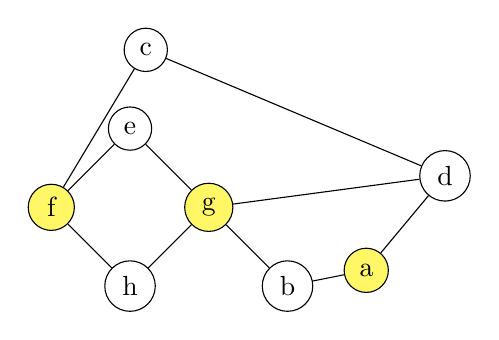
\begin{tikzpicture}
                \node[shape=circle,draw=black, fill=yellow!60] (1) at (0,0) {f};
                \node[shape=circle,draw=black] (2) at (1,1) {e};
                \node[shape=circle,draw=black] (3) at (1,-1) {h};
                \node[shape=circle,draw=black, fill=yellow!60] (4) at (2,0) {g};
                \node[shape=circle,draw=black] (5) at (1.2,2) {c};
                \node[shape=circle,draw=black] (6) at (5,0.4) {d};
                \node[shape=circle,draw=black] (7) at (3,-1) {b};
                \node[shape=circle,draw=black, fill=yellow!60] (8) at (4,-0.8) {a};

                \draw[-] (1) edge node[left] {} (2);
                \draw[-] (1) edge node[left] {} (3);
                \draw[-] (1) edge node[left] {} (5);

                \draw[-] (2) edge node[left] {} (4);
                \draw[-] (3) edge node[left] {} (4);

                \draw[-] (4) edge node[left] {} (6);
                \draw[-] (4) edge node[left] {} (7);

                \draw[-] (7) edge node[left] {} (8);

                \draw[-] (8) edge node[left] {} (6);

                \draw[-] (5) edge node[left] {} (6);
            \end{tikzpicture}
        \end{center}
        \caption{Independent Set formato da $\{f,g,a\}$}
    \end{figure}

    \begin{figure}[H]
        \begin{center}
            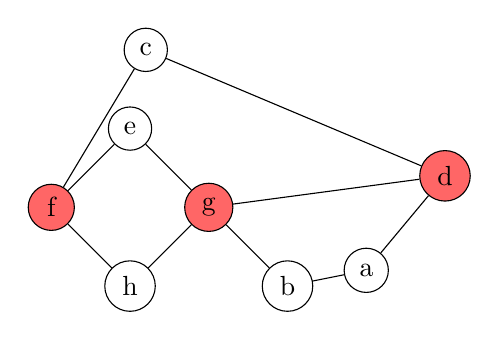
\begin{tikzpicture}
                \node[shape=circle,draw=black, fill=red!60] (1) at (0,0) {f};
                \node[shape=circle,draw=black] (2) at (1,1) {e};
                \node[shape=circle,draw=black] (3) at (1,-1) {h};
                \node[shape=circle,draw=black, fill=red!60] (4) at (2,0) {g};
                \node[shape=circle,draw=black] (5) at (1.2,2) {c};
                \node[shape=circle,draw=black, fill=red!60] (6) at (5,0.4) {d};
                \node[shape=circle,draw=black] (7) at (3,-1) {b};
                \node[shape=circle,draw=black] (8) at (4,-0.8) {a};

                \draw[-] (1) edge node[left] {} (2);
                \draw[-] (1) edge node[left] {} (3);
                \draw[-] (1) edge node[left] {} (5);

                \draw[-] (2) edge node[left] {} (4);
                \draw[-] (3) edge node[left] {} (4);

                \draw[-] (4) edge node[left] {} (6);
                \draw[-] (4) edge node[left] {} (7);

                \draw[-] (7) edge node[left] {} (8);

                \draw[-] (8) edge node[left] {} (6);

                \draw[-] (5) edge node[left] {} (6);
            \end{tikzpicture}
        \end{center}
        \caption{Independent Set Sbagliato }
    \end{figure}

    \[
        MIS = \arg\max_{s} |S|, \forall S \in IS(G)    
    \]

    \begin{figure}[H]
        \begin{center}
            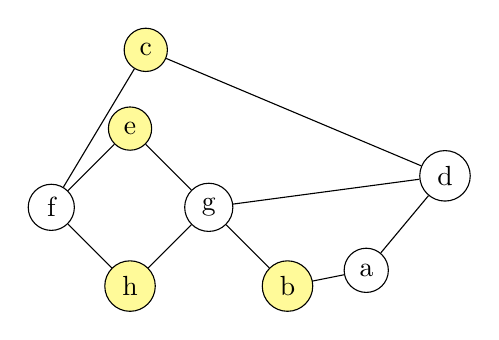
\begin{tikzpicture}
                \node[shape=circle,draw=black] (1) at (0,0) {f};
                \node[shape=circle,draw=black, fill=yellow!40] (2) at (1,1) {e};
                \node[shape=circle,draw=black, fill=yellow!40] (3) at (1,-1) {h};
                \node[shape=circle,draw=black] (4) at (2,0) {g};
                \node[shape=circle,draw=black, fill=yellow!40] (5) at (1.2,2) {c};
                \node[shape=circle,draw=black] (6) at (5,0.4) {d};
                \node[shape=circle,draw=black, fill=yellow!40] (7) at (3,-1) {b};
                \node[shape=circle,draw=black] (8) at (4,-0.8) {a};

                \draw[-] (1) edge node[left] {} (2);
                \draw[-] (1) edge node[left] {} (3);
                \draw[-] (1) edge node[left] {} (5);

                \draw[-] (2) edge node[left] {} (4);
                \draw[-] (3) edge node[left] {} (4);

                \draw[-] (4) edge node[left] {} (6);
                \draw[-] (4) edge node[left] {} (7);

                \draw[-] (7) edge node[left] {} (8);

                \draw[-] (8) edge node[left] {} (6);

                \draw[-] (5) edge node[left] {} (6);
            \end{tikzpicture}
        \end{center}
        \caption{Maximum Independent Set formato da $\{e,h,c,b\}$}
    \end{figure}
\end{definition}

La soluzione per questo problema sfrutta la \textbf{programmazione dinamica}
come approccio. Si risolvono dei sotto-problemi per poi risolvere il problema
principale.

In generale, $MIS$ è $NP-Completo$ e una implementazione Naive richiede $\mathcal{O}(n^2 2^n)$ come complessità temporale. Ma con gli \textbf{alberi} il problema si può risolvere in tempo \textbf{lienare}!

%albero con 1 nodo radice e 3 nodi figli
%per ogni nodo figlio ci sono 2 nodi figli

\begin{figure}[H]
    \begin{center}
        \begin{forest}
            for tree={circle,draw, l sep=20pt}
            [v
                [1, fill=blue!40
                        [1.1, fill=blue!40]
                        [1.2, fill=blue!40]
                ]
                [2, fill=green!40
                        [2.1, fill=green!40
                                [2.1.1, fill=green!40]
                                [2.1.2, fill=green!40]
                        ]
                        [2.2, fill=green!40]
                ]
                [3, fill=red!40
                        [3.1, fill=red!40]
                        [3.2, fill=red!40]
                ]
            ]
        \end{forest}
    \end{center}
\end{figure}

\[
    MIS(v) = \textcolor{red}{MIS(T_{v,1})} + \textcolor{green}{MIS(T_{v,2})} + \textcolor{red}{MIS(T_{v,3})} \pm v
\]

\subsubsection{L'algoritmo di programmazione dinamica}

Per ogni vertice $v$ calcoliamo:
\begin{itemize}
    \item $M^+[v]$ = $|MIS(T_v) \cup \{v\}|$
    \item $M^-[v]$ = $|MIS(T_v) \setminus \{v\}|$
\end{itemize}

Per un vertice $v$ con figli $w_1, \dots, w_kd$:
\begin{itemize}
    \item $M^+[v] = 1 + \sum_{i=1}^d M^-[w_i]$
    \item $M^-[v] = \sum_{i=1}^d \max\{M^+[w_i], M^-[w_i]\}$
\end{itemize}

Quindi:
\[
    MIS(T) = \max{\{M^+[r], M^-[r]\}}
\]

dove con \textbf{T} si intende l'albero completo.

Praticamente, quello che si fa è \textbf{calcolare il MIS per ogni
    sotto-albero} e poi si sommano i risultati per ottenere il \textbf{MIS
    dell'albero completo}.

L'algoritmo, praticamente, parte dalle \textbf{foglie} e risale verso la
\textbf{radice}.

\begin{esempio}(MIS su un albero facile)
\end{esempio}

%albero con 1 nodo radice e 2 nodi figli
%figlio sinistor ha 2 figli
%numerali in ordnie crescente

\begin{figure}[H]
    \begin{center}
        \begin{forest}
            for tree={circle,draw, l sep=20pt}
            [1
                [2
                        [4]
                        [5]
                ]
                [3]
            ]
        \end{forest}
    \end{center}
\end{figure}

Eseguendo l'algoritmo si ottiene:

\begin{itemize}
    \item \textbf{Nodo 4}:
          \begin{itemize}
              \item $M^+[4] = 1$
              \item $M^-[4] = 0$
          \end{itemize}
    \item \textbf{Nodo 5}:
          \begin{itemize}
              \item $M^+[5] = 1$
              \item $M^-[5] = 0$
          \end{itemize}

    \item \textbf{Nodo 2}:
          \begin{itemize}
              \item $M^+[2] = 1$
              \item $M^-[2] = 2$
          \end{itemize}

    \item \textbf{Nodo 3}:
          \begin{itemize}
              \item $M^+[3] = 1$
              \item $M^-[3] = 0$
          \end{itemize}

    \item \textbf{Nodo 1}:
          \begin{itemize}
              \item $M^+[1] = 1+2 = 3$
              \item $M^-[1] = 3$
          \end{itemize}
\end{itemize}

E cosa ci muoviamo in un caso del genere?

%inserisci immagine clique.png

\begin{figure}[H]
    \begin{center}
        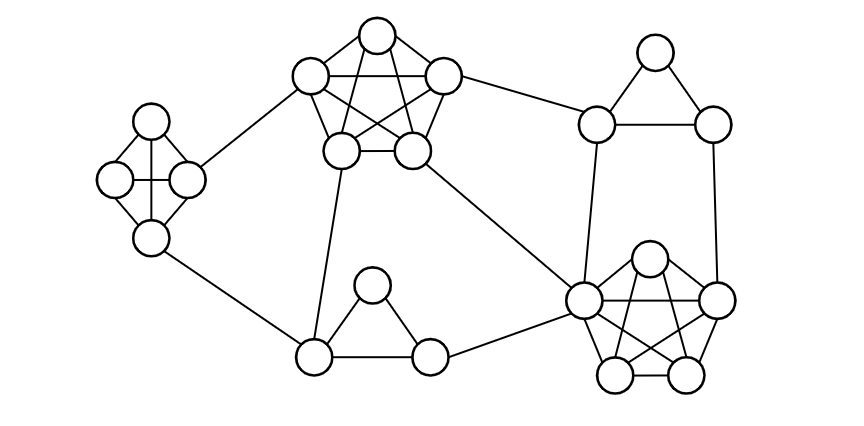
\includegraphics[scale=0.5]{chapters/images/mis clique.png}
    \end{center}
\end{figure}

Se notiamo, possiamo dividere il problema in sotto-problemi.

\begin{figure}
    \begin{center}
        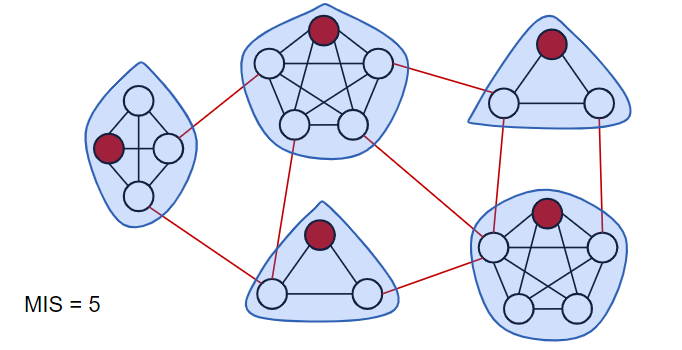
\includegraphics[scale=0.5]{chapters/images/clique format.png}
    \end{center}
    \caption{Formato del problema}
\end{figure}

\textbf{Intuizione}: Possiamo rappresentare un \textbf{grafo} $G$ come un albero $T$. I nodi di $T$ sono dei piccoli
moduli che chiamiamo \textbf{bags}. In questo caso, li trattiamo come \textit{sotto-problemi}.

Utilizziamo la programmazione dinamica per risolvere la tree decomposition.

Copiare grafico di Tree Decomposition: intuition

%disegna un grafo con 9 nodi da 1 a 9
\begin{figure}[H]
    \begin{center}
        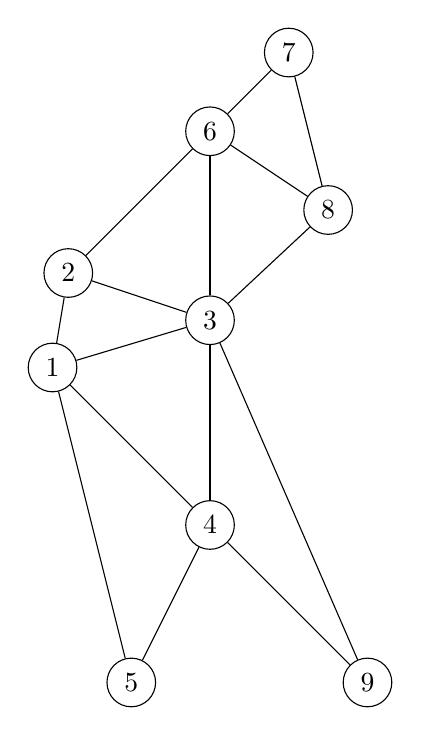
\begin{tikzpicture}
            \node[shape=circle,draw=black] (1) at (0,0) {1};
            \node[shape=circle,draw=black] (2) at (0.2,1.2) {2};
            \node[shape=circle,draw=black] (3) at (2,0.6) {3};
            \node[shape=circle,draw=black] (4) at (2,-2) {4};
            \node[shape=circle,draw=black] (5) at (1,-4) {5};
            \node[shape=circle,draw=black] (6) at (2,3) {6};
            \node[shape=circle,draw=black] (7) at (3,4) {7};
            \node[shape=circle,draw=black] (8) at (3.5,2) {8};
            \node[shape=circle,draw=black] (9) at (4,-4) {9};

            %Ora gli archi
            \draw[-] (1) edge node[left] {} (2);
            \draw[-] (1) edge node[left] {} (3);
            \draw[-] (1) edge node[left] {} (4);
            \draw[-] (1) edge node[left] {} (5);

            \draw[-] (2) edge node[left] {} (6);
            \draw[-] (2) edge node[left] {} (3);

            \draw[-] (3) edge node[above] {} (4);
            \draw[-] (3) edge node[left] {} (9);
            \draw[-] (3) edge node[below] {} (6);
            \draw[-] (3) edge node[left] {} (8);
            %3 edge at 6 but bottom

            \draw[-] (4) edge node [left] {} (9);
            \draw[-] (4) edge node [above] {} (5);

            \draw [-] (6) edge node [left] {} (7);
            \draw [-] (6) edge node [above] {} (8);
            \draw[-] (7) edge node [right] {} (8);

        \end{tikzpicture}
    \end{center}
\end{figure}

\textbf{L'intuizione:} Si prendono praticamente gli insiemi di nodi che formano una \textbf{cricca} tra loro. In questo caso, nel nostro grafo:

\begin{figure}[H]
    \begin{center}
        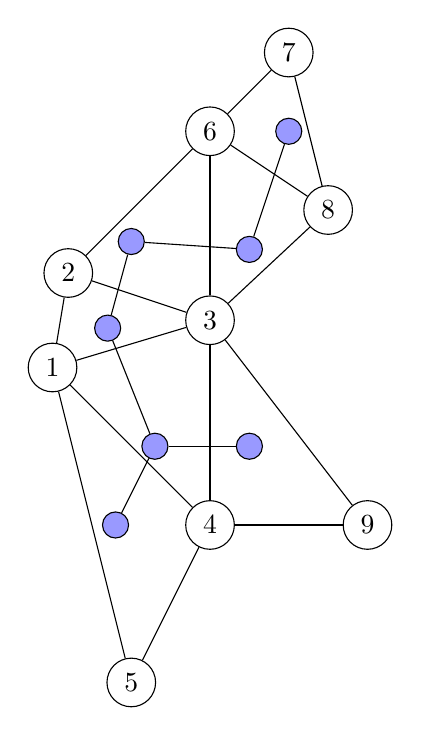
\begin{tikzpicture}
            \node[shape=circle,draw=black] (1) at (0,0) {1};
            \node[shape=circle,draw=black] (2) at (0.2,1.2) {2};
            \node[shape=circle,draw=black] (3) at (2,0.6) {3};
            \node[shape=circle,draw=black] (4) at (2,-2) {4};
            \node[shape=circle,draw=black] (5) at (1,-4) {5};
            \node[shape=circle,draw=black] (6) at (2,3) {6};
            \node[shape=circle,draw=black] (7) at (3,4) {7};
            \node[shape=circle,draw=black] (8) at (3.5,2) {8};
            \node[shape=circle,draw=black] (9) at (4,-2) {9};

            \node[shape=circle,draw=black, fill=blue!40] (a) at (0.7,0.5) {};
            \node[shape=circle,draw=black, fill=blue!40] (b) at (1.3,-1) {};
            \node[shape=circle,draw=black, fill=blue!40] (c) at (0.8,-2) {};
            \node[shape=circle,draw=black, fill=blue!40] (d) at (2.5,-1) {};
            \node[shape=circle,draw=black, fill=blue!40] (e) at (1,1.6) {};
            \node[shape=circle,draw=black, fill=blue!40] (f) at (2.5,1.5) {};
            \node[shape=circle,draw=black, fill=blue!40] (g) at (3,3) {};

            %Ora gli archi
            \draw[-] (1) edge node[left] {} (2);
            \draw[-] (1) edge node[left] {} (3);
            \draw[-] (1) edge node[left] {} (4);
            \draw[-] (1) edge node[left] {} (5);

            \draw[-] (2) edge node[left] {} (6);
            \draw[-] (2) edge node[left] {} (3);

            \draw[-] (3) edge node[above] {} (4);
            \draw[-] (3) edge node[left] {} (9);
            \draw[-] (3) edge node[below] {} (6);
            \draw[-] (3) edge node[left] {} (8);
            %3 edge at 6 but bottom

            \draw[-] (4) edge node [left] {} (9);
            \draw[-] (4) edge node [above] {} (5);

            \draw [-] (6) edge node [left] {} (7);
            \draw [-] (6) edge node [above] {} (8);
            \draw[-] (7) edge node [right] {} (8);

            %archi tra i nodi blu
            \draw[-] (a) edge node[left] {} (b);
            \draw[-] (b) edge node[left] {} (c);
            \draw[-] (b) edge node[left] {} (d);
            \draw[-] (a) edge node[left] {} (e);
            \draw[-] (e) edge node[left] {} (f);
            \draw[-] (f) edge node[left] {} (g);
        \end{tikzpicture}
    \end{center}
\end{figure}

E praticamente si va a formare una \textbf{tree decomposition} di questo tipo:

%Fai un albero che ha valore dei nodi i nodi delle cricche in base ai nodi blu

\begin{figure}[H]
    \begin{center}
        \begin{forest}
            for tree={rectangle,draw, l sep=20pt}
            [{1,2,3}, fill=blue!20
            [{1,3,4}, fill=blue!20
            [{1,4,5}, fill=blue!20]
            [{3,4,9}, fill=blue!20]
            ]
            [{2,3,6}, fill=blue!20
            [{3,6,8}, fill=blue!20
            [{6,7,8}, fill=blue!20]
            ]
            ]
            ]
        \end{forest}
    \end{center}
\end{figure}

\begin{definition}(Tree Decomposition)
    Una tree decomposition di un grafo $G = (V,E)$ è un albero $T$ di bags $X$:
    \begin{itemize}
        \item se $(u,v) \in E$ allora $u$ e $v$ sono nella stessa bag.
        \item $\forall v \in V$ i bags che contengono $v$ sono connessi in $T$
    \end{itemize}

    Un grafo può ammettere diverse tree decomposition.
\end{definition}

\begin{definition}(Tree width)
    La treewidth è la width minore possibile tra tutti le tree decomposition ammesse nel grafo.

    Un po' di notazione:
    \begin{itemize}
        \item $tw(G)$ = treewidth di $G$
        \item $tw(G) = 1 \iff  G$ è una \textbf{foresta}
        \item $tw(G) = 2 \iff G$ è una serie di grafi paralleli
        \item Eliminare un arco in $G$ non aumneta la treewidth
        \item Contrarre archi non aumenta la treewidth
        \item Ogni cricca in $G$ deve essere contenuta in una bag
    \end{itemize}
\end{definition}

\subsection{Cops e Robber}
Abbiamo questo problema che viene definito in questo modo.

\begin{itemize}
    \item \textbf{1 Ladro} che si muove sul grafo.
    \item $k$ poliziotti che si muovono sul grafo.
    \item Per vincere, i poliziotti devono catturare il ladro e arrivare al suo nodo.
\end{itemize}

\begin{theorem}(Cops e Robber Condition)
    $tw(g) \leq k \iff k+1$ poliziotti possono vincere il gioco.

    La strategia è data dalla \textbf{tree decomposition}
\end{theorem}

Usando il grafo di prima, e successivamente anche la tree decomposition che è
stata calcolata prima, possiamo vedere come effettivamente viene risolto il
problema di cops e robber.

\begin{esempio}
    (Cops e Robber)

    %fai una minipage per mettere i due grafi uno accanto all'altro

    \begin{figure}[H]
        \begin{minipage}[t]{0.45\linewidth}
            \centering
            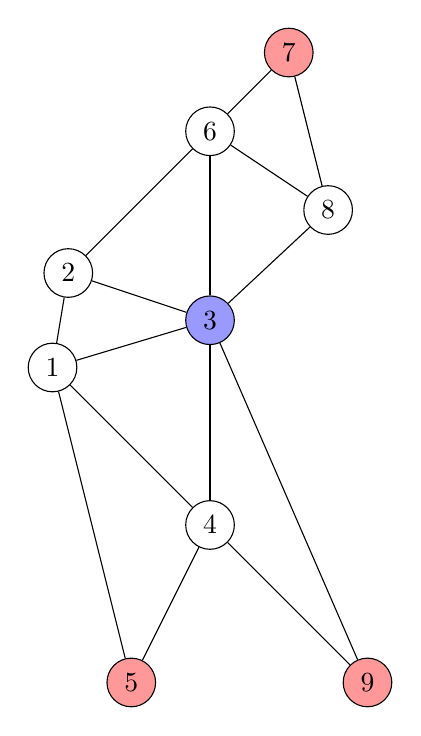
\begin{tikzpicture}

                \node[shape=circle,draw=black] (1) at (0,0) {1};
                \node[shape=circle,draw=black] (2) at (0.2,1.2) {2};
                \node[shape=circle,draw=black, fill=blue!40] (3) at (2,0.6) {3};
                \node[shape=circle,draw=black] (4) at (2,-2) {4};
                \node[shape=circle,draw=black, fill=red!40] (5) at (1,-4) {5};
                \node[shape=circle,draw=black] (6) at (2,3) {6};
                \node[shape=circle,draw=black, fill=red!40] (7) at (3,4) {7};
                \node[shape=circle,draw=black] (8) at (3.5,2) {8};
                \node[shape=circle,draw=black, fill=red!40] (9) at (4,-4) {9};

                \draw[-] (1) edge node[left] {} (2);
                \draw[-] (1) edge node[left] {} (3);
                \draw[-] (1) edge node[left] {} (4);
                \draw[-] (1) edge node[left] {} (5);

                \draw[-] (2) edge node[left] {} (6);
                \draw[-] (2) edge node[left] {} (3);

                \draw[-] (3) edge node[above] {} (4);
                \draw[-] (3) edge node[left] {} (9);
                \draw[-] (3) edge node[below] {} (6);
                \draw[-] (3) edge node[left] {} (8);

                \draw[-] (4) edge node [left] {} (9);
                \draw[-] (4) edge node [above] {} (5);

                \draw [-] (6) edge node [left] {} (7);
                \draw [-] (6) edge node [above] {} (8);
                \draw[-] (7) edge node [right] {} (8);

            \end{tikzpicture}
            \caption{It 1 Grafo}
            \label{fig:tikz}
        \end{minipage}
        \hfill
        \begin{minipage}[t]{0.45\linewidth}
            \centering
            \begin{forest}
                for tree={rectangle,draw, l sep=20pt}
                [{1,2,3}
                    [{1,3,4}
                            [{1,4,5}]
                            [{3,4,9}]
                    ]
                    [{2,3,6}
                            [{3,6,8}
                                    [{6,7,8}]
                            ]
                    ]
                ]
            \end{forest}
            \caption{It 1 Tree Decomposition}
            \label{fig:forest}
        \end{minipage}
    \end{figure}

    In questo caso, la strategia è spostare i \textbf{poliziotti} che sono i nodi
    \textbf{rossi} seguendo la tree decomposition, arrivando a catturare il
    \textbf{ladro} che è il nodo \textbf{blu}.

    \begin{figure}[H]
        \begin{minipage}[t]{0.45\linewidth}
            \centering
            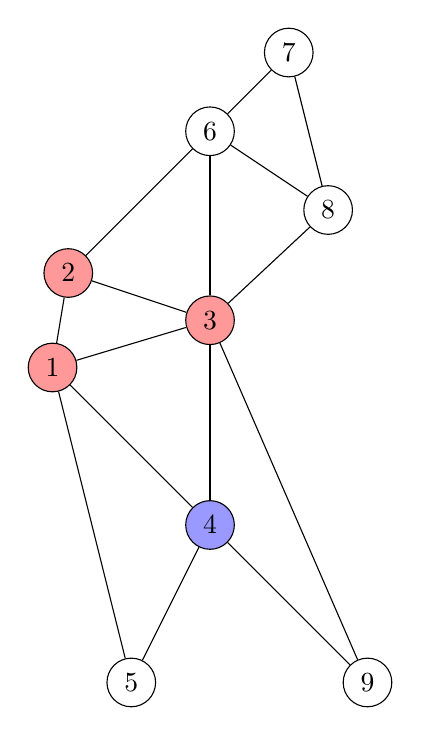
\begin{tikzpicture}
                \node[shape=circle,draw=black, fill=red!40] (1) at (0,0) {1};
                \node[shape=circle,draw=black, fill=red!40] (2) at (0.2,1.2) {2};
                \node[shape=circle,draw=black, fill=red!40] (3) at (2,0.6) {3};
                \node[shape=circle,draw=black, fill=blue!40] (4) at (2,-2) {4};
                \node[shape=circle,draw=black] (5) at (1,-4) {5};
                \node[shape=circle,draw=black] (6) at (2,3) {6};
                \node[shape=circle,draw=black] (7) at (3,4) {7};
                \node[shape=circle,draw=black] (8) at (3.5,2) {8};
                \node[shape=circle,draw=black] (9) at (4,-4) {9};

                \draw[-] (1) edge node[left] {} (2);
                \draw[-] (1) edge node[left] {} (3);
                \draw[-] (1) edge node[left] {} (4);
                \draw[-] (1) edge node[left] {} (5);

                \draw[-] (2) edge node[left] {} (6);
                \draw[-] (2) edge node[left] {} (3);

                \draw[-] (3) edge node[above] {} (4);
                \draw[-] (3) edge node[left] {} (9);
                \draw[-] (3) edge node[below] {} (6);
                \draw[-] (3) edge node[left] {} (8);

                \draw[-] (4) edge node [left] {} (9);
                \draw[-] (4) edge node [above] {} (5);

                \draw [-] (6) edge node [left] {} (7);
                \draw [-] (6) edge node [above] {} (8);
                \draw[-] (7) edge node [right] {} (8);

            \end{tikzpicture}
            \caption{It 2 Grafo}
            \label{fig:tikz}
        \end{minipage}
        \hfill
        \begin{minipage}[t]{0.45\linewidth}
            \centering
            \begin{forest}
                for tree={rectangle,draw, l sep=20pt}
                [{1,2,3}, fill=yellow!40
                [{1,3,4}
                    [{1,4,5}]
                    [{3,4,9}]
                ]
                [{2,3,6}
                    [{3,6,8}
                            [{6,7,8}]
                    ]
                ]
                ]
            \end{forest}
            \caption{It 2 Tree Decomposition}
            \label{fig:forest}
        \end{minipage}
    \end{figure}
    Si continua ad applicare, ogni volta, la strategia in base
    alla tree decomposition.

    \begin{figure}[H]
        \begin{minipage}[t]{0.45\linewidth}
            \centering
            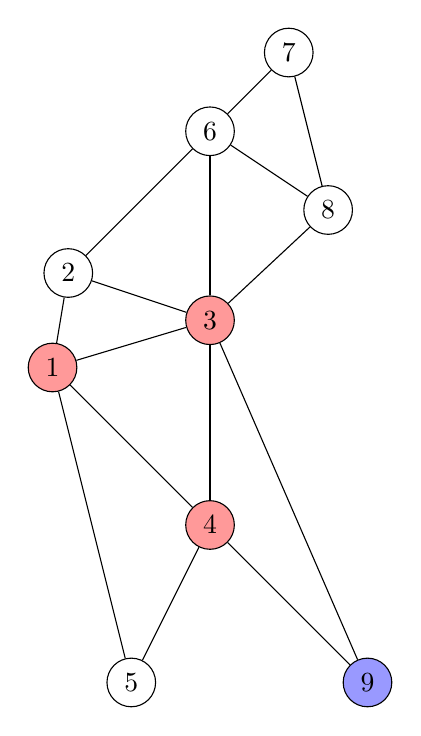
\begin{tikzpicture}
                \node[shape=circle,draw=black, fill=red!40] (1) at (0,0) {1};
                \node[shape=circle,draw=black] (2) at (0.2,1.2) {2};
                \node[shape=circle,draw=black, fill=red!40] (3) at (2,0.6) {3};
                \node[shape=circle,draw=black, fill=red!40] (4) at (2,-2) {4};
                \node[shape=circle,draw=black] (5) at (1,-4) {5};
                \node[shape=circle,draw=black] (6) at (2,3) {6};
                \node[shape=circle,draw=black] (7) at (3,4) {7};
                \node[shape=circle,draw=black] (8) at (3.5,2) {8};
                \node[shape=circle,draw=black, fill=blue!40] (9) at (4,-4) {9};

                \draw[-] (1) edge node[left] {} (2);
                \draw[-] (1) edge node[left] {} (3);
                \draw[-] (1) edge node[left] {} (4);
                \draw[-] (1) edge node[left] {} (5);

                \draw[-] (2) edge node[left] {} (6);
                \draw[-] (2) edge node[left] {} (3);

                \draw[-] (3) edge node[above] {} (4);
                \draw[-] (3) edge node[left] {} (9);
                \draw[-] (3) edge node[below] {} (6);
                \draw[-] (3) edge node[left] {} (8);

                \draw[-] (4) edge node [left] {} (9);
                \draw[-] (4) edge node [above] {} (5);

                \draw [-] (6) edge node [left] {} (7);
                \draw [-] (6) edge node [above] {} (8);
                \draw[-] (7) edge node [right] {} (8);

            \end{tikzpicture}
            \caption{It 3 Grafo}
            \label{fig:tikz}
        \end{minipage}
        \hfill
        \begin{minipage}[t]{0.45\linewidth}
            \centering
            \begin{forest}
                for tree={rectangle,draw, l sep=20pt}
                [{1,2,3}
                [{1,3,4},  fill=yellow!40
                [{1,4,5}]
                [{3,4,9}]
                ]
                [{2,3,6}
                    [{3,6,8}
                            [{6,7,8}]
                    ]
                ]
                ]
            \end{forest}
            \caption{It 3 Tree Decomposition}
            \label{fig:forest}
        \end{minipage}
    \end{figure}

    Ora, seguendo l'ultimo passaggio, si arriva alla fine del gioco e i poliziotti
    hanno vinto.

    \begin{figure}[H]
        \begin{minipage}[t]{0.45\linewidth}
            \centering
            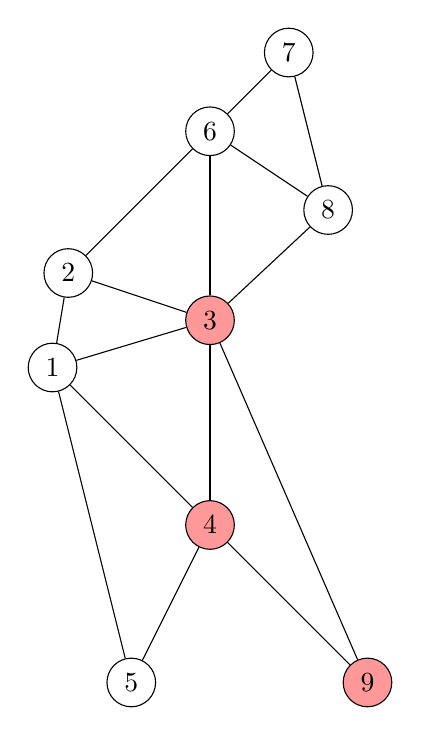
\begin{tikzpicture}
                \node[shape=circle,draw=black] (1) at (0,0) {1};
                \node[shape=circle,draw=black] (2) at (0.2,1.2) {2};
                \node[shape=circle,draw=black, fill=red!40] (3) at (2,0.6) {3};
                \node[shape=circle,draw=black, fill=red!40] (4) at (2,-2) {4};
                \node[shape=circle,draw=black] (5) at (1,-4) {5};
                \node[shape=circle,draw=black] (6) at (2,3) {6};
                \node[shape=circle,draw=black] (7) at (3,4) {7};
                \node[shape=circle,draw=black] (8) at (3.5,2) {8};
                \node[shape=circle,draw=black, fill=red!40] (9) at (4,-4) {9};

                \draw[-] (1) edge node[left] {} (2);
                \draw[-] (1) edge node[left] {} (3);
                \draw[-] (1) edge node[left] {} (4);
                \draw[-] (1) edge node[left] {} (5);

                \draw[-] (2) edge node[left] {} (6);
                \draw[-] (2) edge node[left] {} (3);

                \draw[-] (3) edge node[above] {} (4);
                \draw[-] (3) edge node[left] {} (9);
                \draw[-] (3) edge node[below] {} (6);
                \draw[-] (3) edge node[left] {} (8);

                \draw[-] (4) edge node [left] {} (9);
                \draw[-] (4) edge node [above] {} (5);

                \draw [-] (6) edge node [left] {} (7);
                \draw [-] (6) edge node [above] {} (8);
                \draw[-] (7) edge node [right] {} (8);

            \end{tikzpicture}
            \caption{It Final Grafo}
            \label{fig:tikz}
        \end{minipage}
        \hfill
        \begin{minipage}[t]{0.45\linewidth}
            \centering
            \begin{forest}
                for tree={rectangle,draw, l sep=20pt}
                [{1,2,3}
                    [{1,3,4}
                            [{1,4,5}]
                            [{3,4,9}, fill=yellow!40]
                    ]
                    [{2,3,6}
                            [{3,6,8}
                                    [{6,7,8}]
                            ]
                    ]
                ]
            \end{forest}
            \caption{It Final Tree Decomposition}
            \label{fig:forest}
        \end{minipage}
    \end{figure}
\end{esempio}

\subsection{Calcolare la tree decomposition}

Si usano 2 concetti principali: \textbf{rimuovere un nodo} e
\textbf{triangolazione dei vicini} per costruire le bags.

\begin{definition}(Triangolazione dei vicini e rimozione dei nodi)
    Un grafo $G$ è \textbf{triangolato} se il ciclo più piccolo all'interno del $grafo$ ha lunghezza 3. (Da controllare)
    \begin{figure}[H]
        \begin{center}
            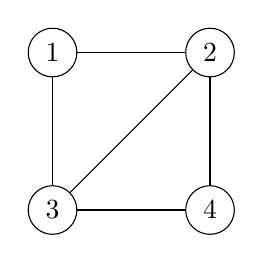
\begin{tikzpicture}
                \node[shape=circle,draw=black] (1) at (0,0) {1};
                \node[shape=circle,draw=black] (2) at (2,0) {2};
                \node[shape=circle,draw=black] (3) at (0,-2) {3};
                \node[shape=circle,draw=black] (4) at (2,-2) {4};

                \path [-] (1) edge node[left] {} (2);
                \path [-] (1) edge node[left] {} (3);
                \path [-] (2) edge node[left] {} (3);
                \path [-] (2) edge node[left] {} (4);
                \path [-] (3) edge node[left] {} (4);
            \end{tikzpicture}
        \end{center}
        \caption{Triangolazione}
    \end{figure}

    Per poter rimuovere un nodo $v$, se nel grafo $G$ rimuoviamo questo $v$, tutti
    i vicini di v $neig(v)$ devono essere tutti connessi tra loro.

    Ad esempio, nel grafo sopra, possiamo rimuovere in un caso il nodo $1$ e nel
    secondo caso il nodo $4$.

    \begin{figure}[H]
        \begin{center}
            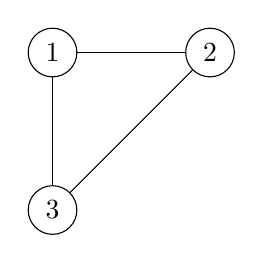
\begin{tikzpicture}
                \node[shape=circle,draw=black] (1) at (0,0) {1};
                \node[shape=circle,draw=black] (2) at (2,0) {2};
                \node[shape=circle,draw=black] (3) at (0,-2) {3};

                \path [-] (1) edge node[left] {} (2);
                \path [-] (1) edge node[left] {} (3);
                \path [-] (2) edge node[left] {} (3);
            \end{tikzpicture}
        \end{center}
        \caption{Triangolazione senza Nodo 4}
    \end{figure}

    \begin{figure}[H]
        \begin{center}
            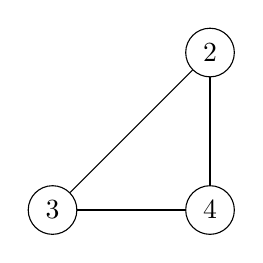
\begin{tikzpicture}
                \node[shape=circle,draw=black] (2) at (2,0) {2};
                \node[shape=circle,draw=black] (3) at (0,-2) {3};
                \node[shape=circle,draw=black] (4) at (2,-2) {4};

                \path [-] (2) edge node[left] {} (3);
                \path [-] (2) edge node[left] {} (4);
                \path [-] (3) edge node[left] {} (4);
            \end{tikzpicture}
        \end{center}
        \caption{Triangolazione senza Nodo 1}
    \end{figure}

    \begin{figure}[H]
        \begin{center}
            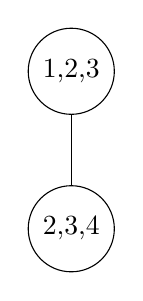
\begin{tikzpicture}
                \node[shape=circle,draw=black] (2) at (0,0) {1,2,3};
                \node[shape=circle,draw=black] (3) at (0,-2) {2,3,4};

                \path [-] (2) edge node[left] {} (3);
            \end{tikzpicture}
        \end{center}
        \caption{Perfect Elimination Order}
    \end{figure}

    I nodi che possono essere rimossi si chiamano \textbf{simplicial node}.

    Quindi, la migliore tree decomposition con la migliore treewidth si riduce a
    trovare la \textbf{PEO} (Perfect Elimination Order)
\end{definition}

Torniamo ora al \textbf{calcolo} della tree decomposition. Partiamo da un
\textbf{removal order} per un grafo.

Disegnare il grafo o mettere qualcos
\[
    removal\_order = [6,7,9,1,8,2,0,3,5,4]
\]

Praticamente, $\forall v \in removal\_order$: rimuovi $v$ e triangola i vicini.
Se i vicini sono già triangolati, si $crea$ la $bag$ che avrà $v$ e i suoi
vicini come nodi.

Si parte questo grafo in foto e mano a mano si cominciano a togliere nodi in
base a quell'ordine indicato.

\begin{figure}[H]
    \begin{center}
        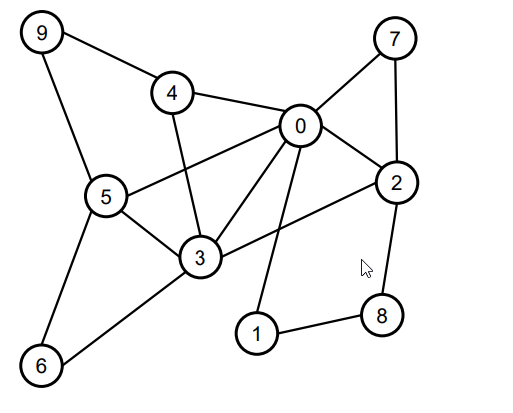
\includegraphics[scale=0.5]{chapters/images/Grafopertree.png}
    \end{center}
    \caption{Grafo iniziale}
\end{figure}

Ad esempio, se si partisse dal nodo $6$ si avrebbe \textbf{rimuovendolo} i suoi
vicini $5$ e $3$ sarebbero già triangolati, ovvero connessi tra loro. Quindi,
siccome non serve fare altro, si crea la bag $\{6,5,3\}$

\begin{figure}[H]
    \begin{center}
        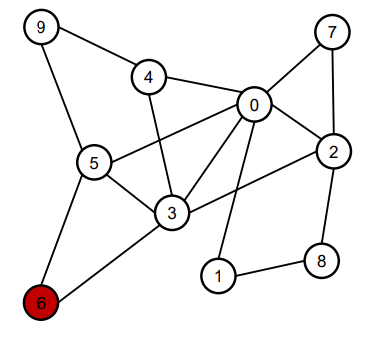
\includegraphics[scale=0.5]{chapters/images/esrimozioen.png}
    \end{center}
    \caption{Esempio rimozione nodo 6}
\end{figure}

%Scrivi un'equazione che spiega che fino a quando non finisci
%il removal order:
%- rimuovi il nodo
%- i vicini sono già triangolati?
%non fai niente
% altrmenti triangoli

\begin{equation}
    \forall v \in removal\_order:
    \begin{cases}
        \text{Rimuovi il nodo}                \\
        \text{I vicini sono già triangolati?} \\
        \begin{cases}
            \text{Si: non fare niente} \\
            \text{Altrimenti: triangola i vicini}
        \end{cases}
    \end{cases}
\end{equation}

\textbf{Nota:} Quando si arriva a $\{3,4,5\}$ notiamo che esise già una bag più grande che è $\{0,3,4,5\}$ e non ci serve
quindi crearne un'altra. Dopo aver creato tutte le bag, \textbf{si connette ogni bag} con la quale l'intersezione è massimale. Cioè, ogni bag è connessa a quell'altra
bag tale che il numero di nodi in comune è massimo.

\begin{figure}[H]
    \begin{center}
        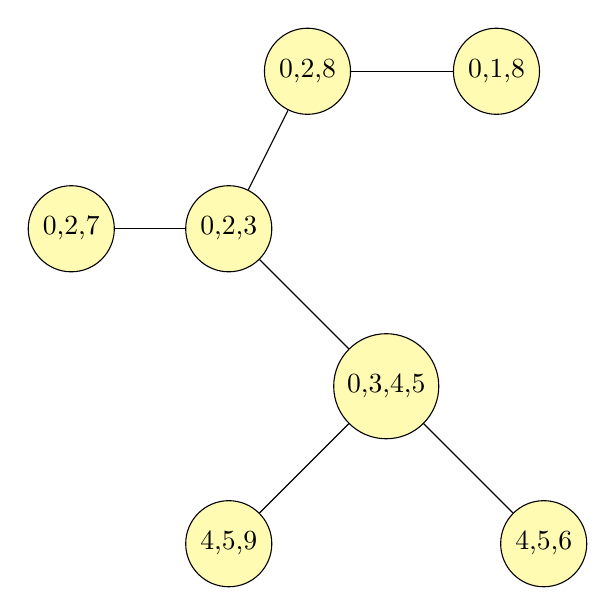
\begin{tikzpicture}
            \node[shape=circle,draw=black, fill=yellow!30] (1) at (0,0) {0,2,7};
            \node[shape=circle,draw=black, fill=yellow!30] (2) at (2,0) {0,2,3};
            \node[shape=circle,draw=black, fill=yellow!30] (3) at (3,2) {0,2,8};
            \node[shape=circle,draw=black, fill=yellow!30] (4) at (5.4,2) {0,1,8};
            \node[shape=circle,draw=black, fill=yellow!30] (5) at (4,-2) {0,3,4,5};
            \node[shape=circle,draw=black, fill=yellow!30] (6) at (2,-4) {4,5,9};
            \node[shape=circle,draw=black, fill=yellow!30] (7) at (6,-4) {4,5,6};

            %Archi

            \draw[-] (1) edge node[left] {} (2);
            \draw[-] (2) edge node[below left] {} (3);
            \draw[-] (3) edge node[left] {} (4);
            \draw[-] (2) edge node[above left] {} (5);
            \draw[-] (5) edge node[above right] {} (6);
            \draw[-] (5) edge node[above left] {} (7);
        \end{tikzpicture}
    \end{center}
    \caption{Tree Decomposition dal Removal Order}
\end{figure}

\textbf{Risultato:} Abbiamo ottenuto una tree decomposition!

La domanda ora è: \textbf{Come otteniamo il \textit{removal order}}?

Il \textbf{calcolo} del removal order è un problema \textbf{NP-Hard}. Ci sono
$N!$ possibili ordini e $\mathcal{O}(2^n)$ con la programmazione dinamica.

Per risolvere questo problema, quindi, è usare un'euristica per trovare delle
\textbf{soluzioni accettabili}.

\begin{definition}(Minimum degree heuristic)
    Quando rimuoviamo un nodo dalla tree decomposition, rimuoviamo il nodo che ha il \textbf{grado minore}, cioé il nodo
    che ha il \textbf{minor numero di vicini}.

    Rimuovere un nodo cambia anche il \textbf{grado} dei vicini e quindi calcoliamo
    il \textbf{minimum degree} ad ogni iterazione.
\end{definition}

Di fatto, il removal order di prima è stato calcolato sfruttando questa
\textbf{minimum degree heuristic}. \newpage